
% Use the article class with font size 11pt
\documentclass[10pt]{article}

% Creates placeholder text (Only needed for this example)
%\usepackage{blindtext}

% Markdown in your latex sounds fun
%\usepackage[footnotes,definitionLists,hashEnumerators,smartEllipses, hybrid]{markdown}

% Float images where you want them
\usepackage{float}

% Deal with language and encoding
\usepackage[T1]{fontenc}
\usepackage[utf8]{inputenc}
\usepackage[english]{babel} 

% setup page size
\usepackage{geometry}
\geometry{a4paper,margin=1.5in,lmargin=1in,rmargin=1in} % reduced margins

% Set up fancy headers and footers
\usepackage{fancyhdr} 
\pagestyle{fancy} % options: empty , plain , fancy
\renewcommand{\headrulewidth}{1pt} % adds line at the bottom of the header

% Set up table of contents
\usepackage[nottoc,notlof,notlot]{tocbibind}
\usepackage[titles,subfigure]{tocloft}

% Set up graphics and figures
\usepackage{graphicx}
\usepackage{wrapfig}
\usepackage{subcaption} % subfigure and subfig are also options

% Better tables in latex
\usepackage[table,xcdraw]{xcolor}
\usepackage{booktabs} 
\usepackage{multirow}

% Begin paragraphs with an empty line rather than an indent
\usepackage[parfill]{parskip}

% For including code 
%\usepackage{verbatim}
\usepackage{listings}
\usepackage{color}

% Setup colors for code highlighting
\definecolor{commentcolor}{rgb}{0,0.4,0}
\definecolor{stringcolor}{rgb}{0.5,0.8,0.5}
\definecolor{identifiercolor}{rgb}{0.1,0.1,0.1}
\definecolor{keywordcolor}{rgb}{0.2,0,0.9}

\definecolor{numbercolor}{rgb}{0.5,0.5,0.5}
\definecolor{backgroundcolor}{rgb}{0.975,0.975,0.975}

% Setup style of code listings
\lstset{
    breakatwhitespace=false,
    breaklines=true,
    commentstyle=\itshape\color{commentcolor},
    frame=leftline,
    backgroundcolor=\color{backgroundcolor},
    keepspaces=true,
    keywordstyle=\bfseries\color{keywordcolor},
    identifierstyle=\color{identifiercolor},
    numbers=left,
    numbersep=10pt,
    numberstyle=\small\color{numbercolor},
    rulecolor=\color{black},
    showspaces=false,
    showstringspaces=false,
    showtabs=false,
    stepnumber=1,
    stringstyle=\color{stringcolor},
    tabsize=2,
    title=\lstname
}

% Better maths rendering
\usepackage{array}

% For more list types
\usepackage{paralist}

%
\usepackage{enumitem}

%
\usepackage{multicol}

%
\usepackage{pdflscape}

% Better section formatting
\usepackage{sectsty}

% lazy formatting of 1st, 2nd, 3rd
\usepackage[super,negative]{nth}

% Sets up formatting for section headings
\allsectionsfont{\sffamily\mdseries\upshape}
\renewcommand{\cftsecfont}{\rmfamily\mdseries\upshape}
\renewcommand{\cftsecpagefont}{\rmfamily\mdseries\upshape}

% Set up header and footer text
\makeatletter
\lhead{\@title}\chead{}\rhead{\@author}
\lfoot{}\cfoot{\thepage}\rfoot{}
\makeatother

% Should show blue underlines on links, but it doesn't appear to work
\usepackage[colorlinks=false, allbordercolors={0 0 0}, linkbordercolor=blue, pdfborderstyle={/S/U/W 1}]{hyperref}

% Tell latex that your images are in a folder called Images
\graphicspath{{Images/}}

% Use url for better url handling
\usepackage{url}

% Use biblatex for citations
\usepackage{csquotes}
\usepackage[
    backend=biber,
    style=numeric,
    sorting=ynt
]{biblatex}
\addbibresource{references.bib}

% My custom title page package
\usepackage{UoYTitlePage}


%%% =====================================================
%%% =====================================================
%%%     You Should Only Have To Edit Stuff Below
%%%     Here. Unless You Want To Change The Style.
%%% =====================================================
%%% =====================================================


% ====================================
% Set up tile, author and other stuff
% ====================================

\uni{University of York}
\dept{Department of Electronics}

\module{Biologically Inspired Computation}
\project{Neural Networks For\\Speech Interaction}

\title{Eco-Res Project}
\author{Zak West}

\supervisor{ }
\logo{logo}

\abstracttext{
The history and technology behind speech based human computer interfaces, and the role neural networks play in current implimentations.
}

% ====================================
% Start of the main document
% ====================================
\begin{document}
    
	% ============
	% Title Page
	% ============
	\maketitle
	
	% ============
	% Contents Page
	% ============
	%\pagenumbering{roman} % Use roman numerals for page numbers
	%\tableofcontents % Adds a table of contents
	%\listoffigures % Adds a list of figures
	%\newpage
	\pagenumbering{arabic} % Use Arabic (integer) numbering

	% ============
	% Main Pages
	% ============
    	
	\section*{What is a neural network}
	    
	    \begin{figure}[H]
            \centering
            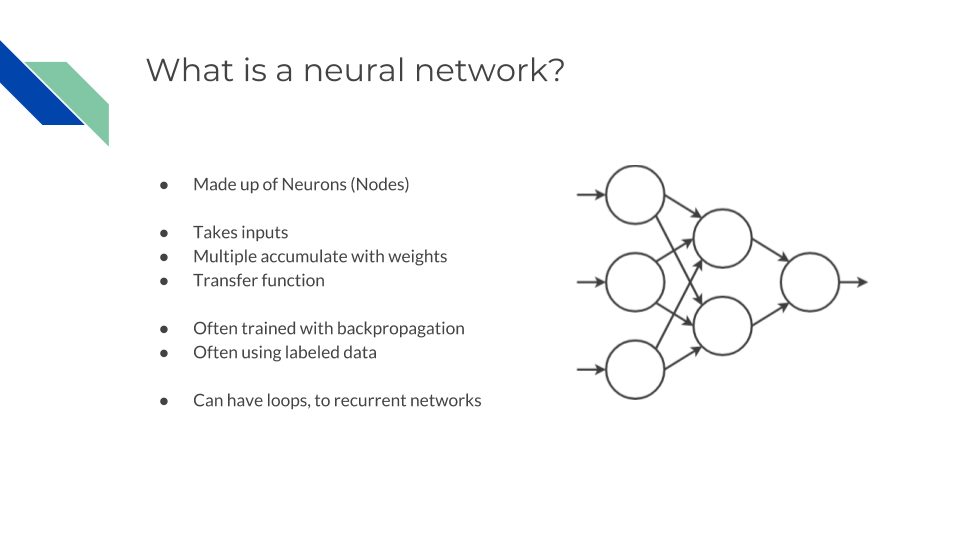
\includegraphics[width=1\textwidth]{slide_1}
            \label{fig:appendix:slide_1}
        \end{figure}
        
        Neural networks are a type of machine learning, pioneered in the 1940s by McCulloch and Pitts. 
        
        They are made up of multiple neurons (or nodes), that are structured into layers. Each neuron has one or more inputs and a set of weights associated with them. These neurons operate by applying a simple process to their inputs to create an output. Each neuron takes its inputs and multiplies them by the associated weights and then applies a transfer function. This transfer function may be a binary step, sigmod, or tanh to name a few.  
        
        The thing that makes Neural networks special is that they can be trained, or taught.  This can be done in many ways, but the simplest is using labelled data and backpropagation. This approach uses the correct output values and alters the weights of the neurons to get the network to agree. 
        
        Neural networks can have this simple structure, but they often have more complex structures. such as backwards connections from one layer to the previous. This is known as recurrence and is one tool used for speech recognition.  They can also be modified to accept complex inputs like audio or even images, this normally done using convolution neural networks.


        \newpage

    \section*{History of Voice based AI assistants}
	    
	    \begin{figure}[H]
            \centering
            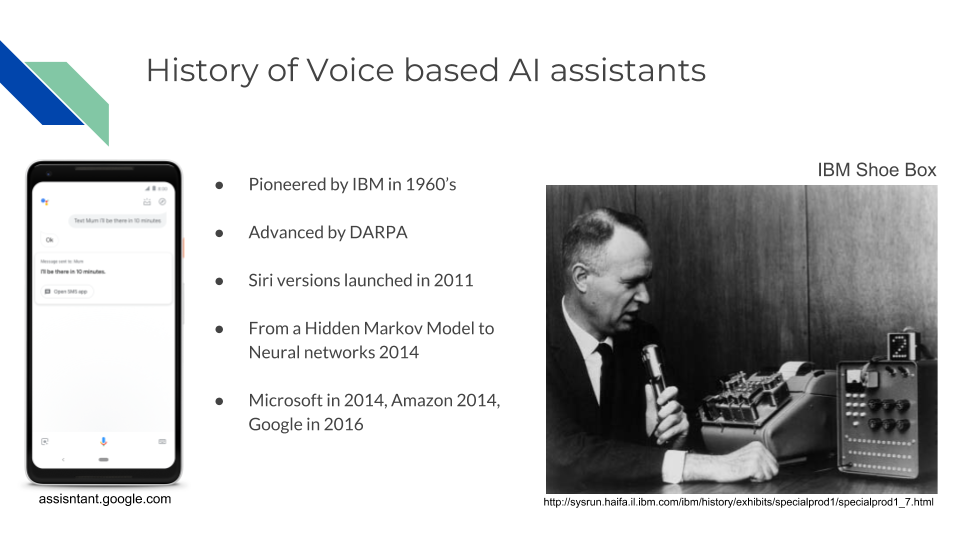
\includegraphics[width=1\textwidth]{slide_2}
            \label{fig:appendix:slide_2}
        \end{figure}
        

        Speech-based human-computer interfaces have a surprisingly long history.  Which starts off around the '50s, below some of these are listed. 
        
        In 1953 Bell Labs created a system called Audrey, which could recognise spoken digits.\cite{juang2005automatic}
        It used the differences in resonance that different vowel sounds produce to classify digits.\cite{davis1952automatic}

                In 1961 IBM unveiled a device at the Seattle worlds fair called the “shoebox”\cite{shoebox}, This device was, as you may have guessed, about the size of a shoe box. 
        It allowed people to perform arithmetic using voice commands by saying digits and commands words such as “plus” or “minus”. It would then illuminate the correct light as an output. It was implemented using 3 filters and discreet logic.
        
        In the ’70s DARPA created a tool called Harpy that could recognise around a thousand words. \cite{1976PhDT........81L}
        
         By the ’80s this team had developed the system to not only recognise words but phrases, using hidden Markov models \cite{rabiner1986introduction}. These models can be thought of as a kind of probabilistic Finite state machine.

        In the ’90s this technology started to appear for personal computers, with the main players being Microsoft and IBM.

        But it wasn't till 2011 and the introduction of Siri\cite{siri} to the iPhone that this technology became widespread. Siri was originally developed by a spin-out company from DARPA (again) and it still used hidden Markov models. It wasn't until 2014 that neural networks were used for Siri. \cite{wired}. Siri now uses many advanced ANN techniques such as CNNs, DNNs and RNNs.
        
        Now there are many competitors to Siri. Such as Microsoft's Cortana or Amazon's Alexa.
        \newpage

    \section*{CNN and DNN}
	    
	    \begin{figure}[H]
            \centering
            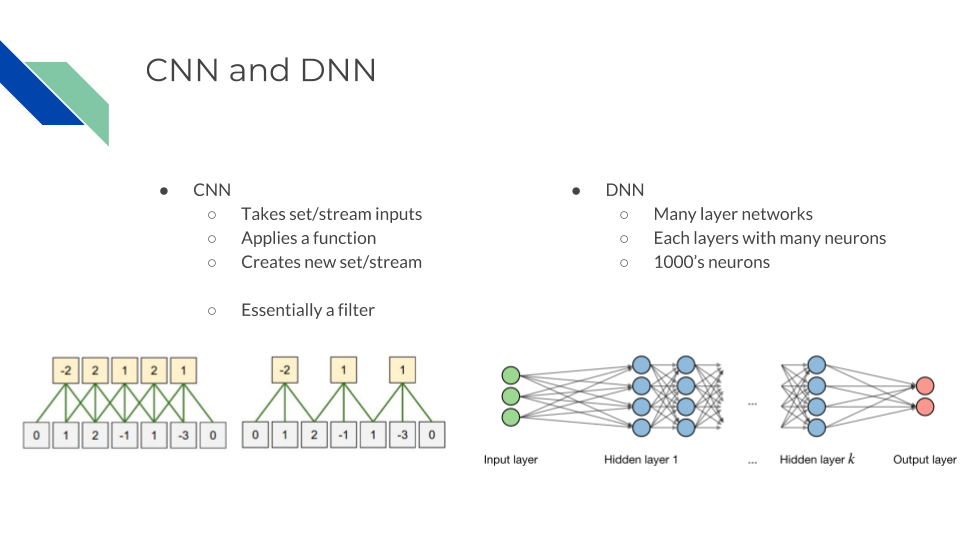
\includegraphics[width=1\textwidth]{slide_3}
            \label{fig:appendix:slide_3}
        \end{figure}
         Now, most voice assistants are using Convolution neural networks on time series inputs.\cite{LeCun1998-nt}
        
        Convolution itself is the process of taking multiple input variables (in this case the last few audio samples) and applying a function ( aka a kernel)  to them to get a new waveform.  A simple convolution in images is to detect edges. You know you have an edge if the pixel to your left is black and the one to your right is white. For audio a simple convolution can be low pass filter, the convolution function make the current output the average of the last few inputs. This removes fast changes, thus removing high frequencies.
        These can also provide a time delay to a signal.
        
         In general, CNNs tend to have multiple of these filters. With each one being trained to apply a different filter to the input. 
        
        These may also change the sample rate of the data as it gets further into the network because more complicated features span longer amounts of time. A phoneme has a longer duration than the frequencies that make it up and a word takes longer than the phonemes that make it up. Changing this sample rate allows you to have a lot fewer neurons in later layers, which make the networks smaller and faster.
                        
        
        DNNs are deep neural networks. 
        It wasn't long after the first neural networks were proposed that multilayer networks were created, in 1965 the first paper was published on them \cite{ivakhnenko1965cybernetic}.  Here deep refers to many layers.
        Modern deep neural networks can have 100s of layers and potentially thousands of nodes. This allows for the networks to represent more complex and higher order functions. As well as higher levels representing more complex ideas.
        Deep neural networks can also contain many different types of network. I.e they could have and input convolutional network then a feed forward. Or an LSTM and then a feedforward

        \newpage

    \section*{RNN and LSTM}
	    
	    \begin{figure}[H]
            \centering
            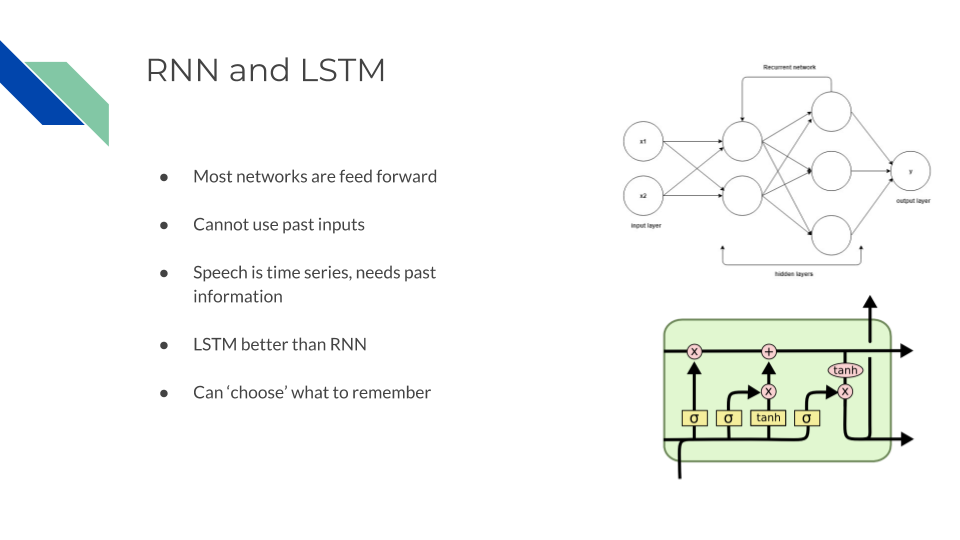
\includegraphics[width=1\textwidth]{slide_4}
            \label{fig:appendix:slide_4}
        \end{figure}

        RNNs are recurrent neural networks. This means there is some form of backwards connection in the network.  This means that the previous state of the network can affect the next state.  These were first proposed by John Hopfield in 1982 \cite{hopfeild}. This is a very useful feature to have when working with time series data like speech. As it is very common for the previous inputs to affect the current state.
        Unfortunately, RNNs have a problem. Feedback. This causes vanishing or exploding gradients and outputs. Which make them very hard to train. RNNs also constantly update their state with the new input, this means they're not very good when something from a long time ago should influence the current state. I.e a couple of words back or the previous sentence. 

        A new architecture of RNNs was proposed in 1997\cite{lstm} called LSTM, which was then improved in 1999\cite{forget}
        LSTMs fix this by allowing the network to choose how much it remembers of the current state by using multiple gates for each unit. This means each LSTM cell can remember only important cues. This also fixes the gradient problem.
        
        LSTM have been shown to be very good at a wide array of time series prediction and classification tasks, including dealing with voice.

        \newpage

    \section*{Natural language processing}
	    
	    \begin{figure}[H]
            \centering
            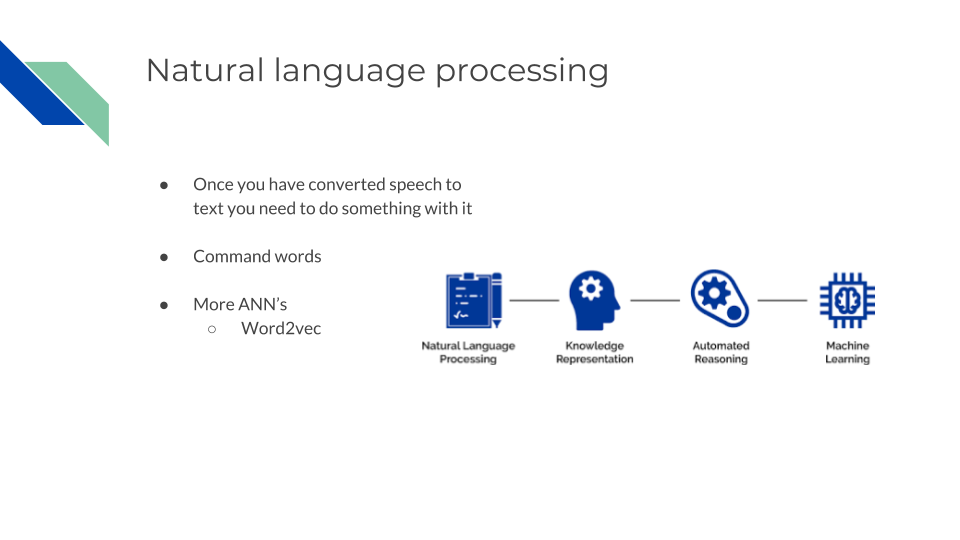
\includegraphics[width=1\textwidth]{slide_5}
            \label{fig:appendix:slide_5}
        \end{figure}

         Once you have converted that speech to text you have to do something with it. This is where natural language processing comes in.
        The simplest way of doing this is using command words. This is what the IBM shoe box from earlier did. In that case, the command words were "plus" or "add". 
        This is still used, for simple phrases like "turn the music down". But that isn't very natural for people and it would be hard to enumerate every possible command.
        
        The next step is using rules based approaches. These don't depend on exact matches, but still tend to have limited numbers of known phrases. Phrases such as "schedule a meeting at 4pm with John" can be done with rules based approaches. \cite{nlp}
        
        Since the '80s ANNs are also used to do this. This is a statistical approach to NLP. Currently LSTMs are often used because they are good with sequences. Representing words in an ANN is quite a difficult task there are many methods but the most popular at the moment is Word2Vec which uses vectors to map to words. \cite{mikolov2013efficient}
        
        \newpage

    \section*{Future?}
	    
	    \begin{figure}[H]
            \centering
            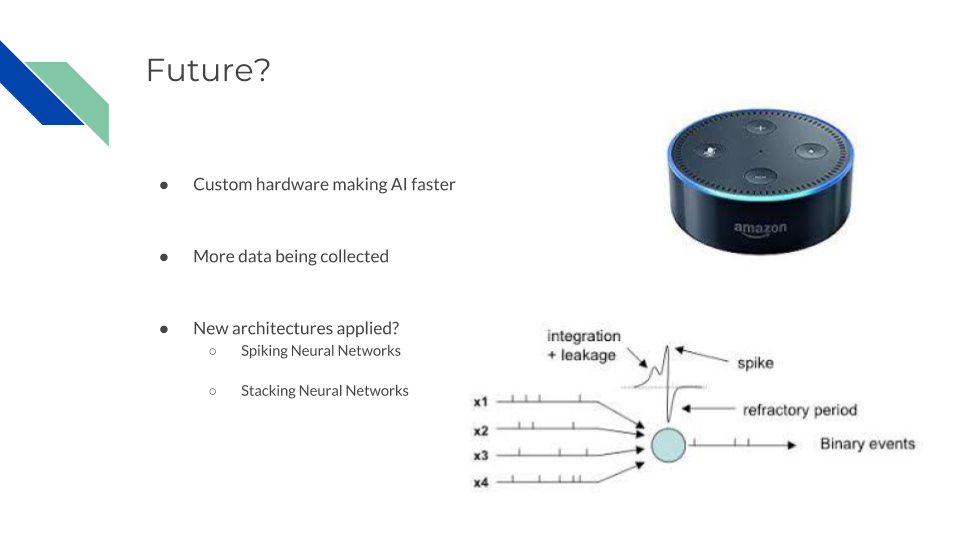
\includegraphics[width=1\textwidth]{slide_6}
            \label{fig:appendix:slide_6}
        \end{figure}

        Currently, custom devices are being created and sold, whose primary function I speech interaction. These are the Amazon echo, Google Home and the Apple HomePod.
        
        These devices currently use tradition computer hardware. Most likely ARM CPUs. But since they are single-purpose devices they could start to use custom chips with dedicated ANN and DSP functionality. The speed improvements from this would be massive and so networks could be able to be made more complex.
        
        There is also interest in using spiking neural networks and other models based more directly off of real neurons\cite{tsai2017always}. The idea is that these networks are continuous in the time domain. This is maybe an advantage when processing continuous time domain data like speech.

        \newpage
    % ============
	% Bibliography Pages
	% ============
	\vspace{6cm}
	\printbibliography


\end{document}
